Pro potřeby této práce byly vytvořeny 2 aplikace a~2 knihovny. První aplikace
je demonstrační aplikací k~měřicímu vozu a~pouze zobrazuje naměřená data. Druhá
aplikace je o~mnoho komplexnější a~řeší přímo problém automatické kalibrace.

\section{Volba nástrojů}
\label{sec:sw-nastroje}

Zásadní otázkou, kterou je třeba zodpovědět před vytvářením programu, je,
jaký programovací jazyk a~případně framework zvolit. Zde měl autor poměrně
jasný požadavek na programovací jazyk: jazyk musí mít poměrně silný typový
systém tak, aby netriviální množství kontrol proběhlo již během překladu.
Důvodem pro tento argument je fakt, že autor vyrábí aplikaci, které je tzv.
\textit{kritická}. V~kontextu této práce to znamená, že vlivem chyby
v~aplikaci může dojít k~materiálním škodám na kalibrovaném modelu (ceny
vybraných malosériových modelů se pohybují až v~desítkách tisíc Kč).

Dalším přirozeným požadavkem bylo, aby programovací jazyk měl rozumnou podporu
pro komunikaci se sériovým portem, neboť toto rozhraní bude použito jak pro
komunikaci s~měřicím vozem, tak pro komunikaci s~digitální centrálou \gls{DCC}.

Dalším kritériem při výběru programovacího jazyka byla jeho předchozí znalost
autorem práce. Zejména u~kritických aplikací je totiž nanejvýš důležité, aby
programátor přesně věděl, co dělá.

Při zvažování technologií aplikace bylo rozhodnuto, že program by měl
mít grafické uživatelské rozhraní (GUI), neboť je nanejvýš vhodné zobrazovat
přehledně aktuální průběh kalibrace a~neboť jsou běžní uživatelé na GUI
aplikace zvyklí.

Zásadní je pak otázka typu aplikace. Autor uvažoval aplikace desktopové,
mobilní, webové a~dokonce i~embedded! Embedded aplikace s~sebou nesou tu
nevýhodu, že obsluha s~aplikací typicky nemůže příliš interagovat, u~mobilních
aplikací je v~kontextu této práce omezující zejména zobrazovací plocha
zařízení, na kterou se jednoduše nevejde tolik dat, kolik by aplikace chtěla
zobrazovat. Navíc vývoj pro jiné zařízení, než na kterém se kód píše, vždy
přináší nějakou režii navíc.

Výhodou webové aplikace by byla snadná přenositelnost na jiné počítače,
aplikace by dokonce mohla být přístupná i~z~mobilního zařízení. Bohužel, proti
tomuto formátu aplikace hovoří fakt, že autor práce nemá s~webovými aplikacemi
dostatečné zkušenosti a~už vůbec si netroufá v~nich psát kritický kód.
Oproti desktopovým aplikacím jsou interaktivní webové aplikace navíc o~něco
složitější (zejména co se týče předávání signálů z~GUI).

Další možností pak byly desktopové aplikace. Vzhledem k~požadavkům uvedeným
výše a~k~faktu, že se jedná už o~poněkud rozsáhlejší projekt, jako nejvhodnější
se autorovi jevil jazyk \texttt{C++} s~použitím frameworku \texttt{Qt}.
Argumentem pro tento framework byly dobré osobní reference, které na
\texttt{Qt} autor práce dostal od kolegů. Ukázalo se také, že \texttt{Qt} poskytují
nejen výbornou multiplatformní podporu pro GUI, ale také stejně dobrou
multiplatformní podporu pro sériový port. Bylo tedy rozhodnuto, že výsledná
aplikace bude psána v~programovacím jazyce \texttt{C++} (konkrétně
\texttt{C++14}) za použití frameworku \texttt{Qt} a~bude multiplatformní
(minimálně mezi OS \texttt{Windows} a~\texttt{Linux}).

\section{\gls{WSM} Speed Reader}
\label{sec:sw-wsm-speed-reader}

První aplikací je \textit{\gls{WSM} Speed Reader}\footnote{\gls{WSM} je obchodní název
vyvinutého měřicího vozu: \textit{\gls{WSM}: A~Wireless Speedometer}.} -- jednoduchý
zobrazovač vyčtených dat. Aplikace se skládá z~jednoho okna a~je především typu
\textit{proof of concept}. GUI aplikace je zachyceno na obrázku
\ref{fig:wsm-speed-reader-gui}.

\begin{figure}[ht]
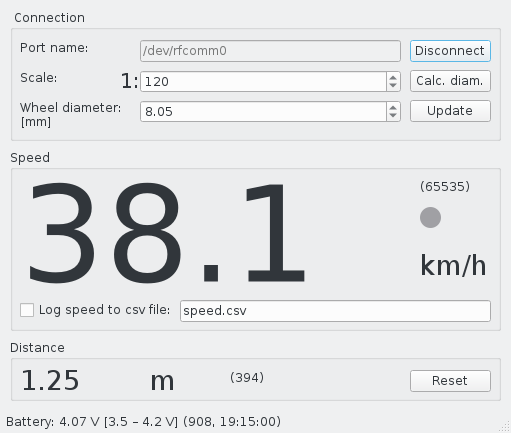
\includegraphics[width=0.7\textwidth]{data/speed_reader_screenshot.png}
\caption{GUI programu \gls{WSM} Speed Reader.}
\label{fig:wsm-speed-reader-gui}
\end{figure}

Aplikace se připojuje k~sériovému portu, ze zadaných parametrů vypočítává
rychlost a~ujetou vzdálenost vozidla a~tyto údaje zobrazuje. Umožňuje ukládání
vyčtených dat do souboru (především pro vývoj) a~ukládání nastavení aplikace
do konfiguračního souboru. Aplikace je volně dostupná pod licencí Apache
License v2.0 \cite{wsm-speed-reader}.

Při programování této aplikace bylo rozhodnuto vyčlenit knihovnu umožňující
komunikaci s~měřicím vozem \gls{WSM} do samostatného repozitáře. Knihovna se skládá
hlavičkového souboru \texttt{wsm.h}, který definuje API třídy \texttt{Wsm},
implementace této knihovny (v~samostatném \texttt{cpp} souboru) a~pomocných
souborů. Knihovna je k~dispozici
online\footnote{\url{https://github.com/kmzbrnoI/wsm-lib-cpp-qt}}, bylo k~ní
vytvořeno srozumitelné README a~dodány všechny náležitosti samostatně stojícího
projektu.

I~přes původní snahy je nutné pro užití knihovny v~projektu využít frameworku
\texttt{Qt} a~to zejména kvůli implementaci sériového portu.


\newpage
\section{Automatic Calibration}
\label{sec:sw-wsm-auto-calib}

Program \textit{Automatic Calibration} umožňuje automaticky provést proces
kalibrace. V~souladu s~požadavky kladenými na výsledné sofwarové řešení
umožňuje

\begin{compactitem}
\item připojení k~XpressNET centrále a~měřicímu vozu \gls{WSM},
\item ruční řízení libovolného hnacího vozidla,
\item vyčítání základních \gls{CV} (viz \ref{sec:trendy}) lokomotivy,
\item načtení závislosti \textit{jízdní stupeň -- rychlost} ze
souboru\footnote{Tato závislost je úzus a~je typicky jediná v~rámci
modelářského klubu či většího celku. V~KMŽ Brno~I je používána závislost
definovaná v~příloze \ref{fig:step-to-speed}.},
\item plně automatickou kalibraci rychlostní tabulky,
\item poloautomatickou kalibraci hodnoty decelerace,
\item konfiguraci parametrů kalibrace konfiguračním souborem,
\item zobrazení průběhu kalibrace, přerušení a~obnovení kalibrace,
\item načtení a~uložení profilu lokomotivy do souboru,
\item zobrazení grafu závislosti rychlosti na otáčkách motoru.
\end{compactitem}

Grafické uživatelské rozhraní aplikace je zachyceno na obrázku \ref{fig:ac-gui}.

\begin{figure}[ht]
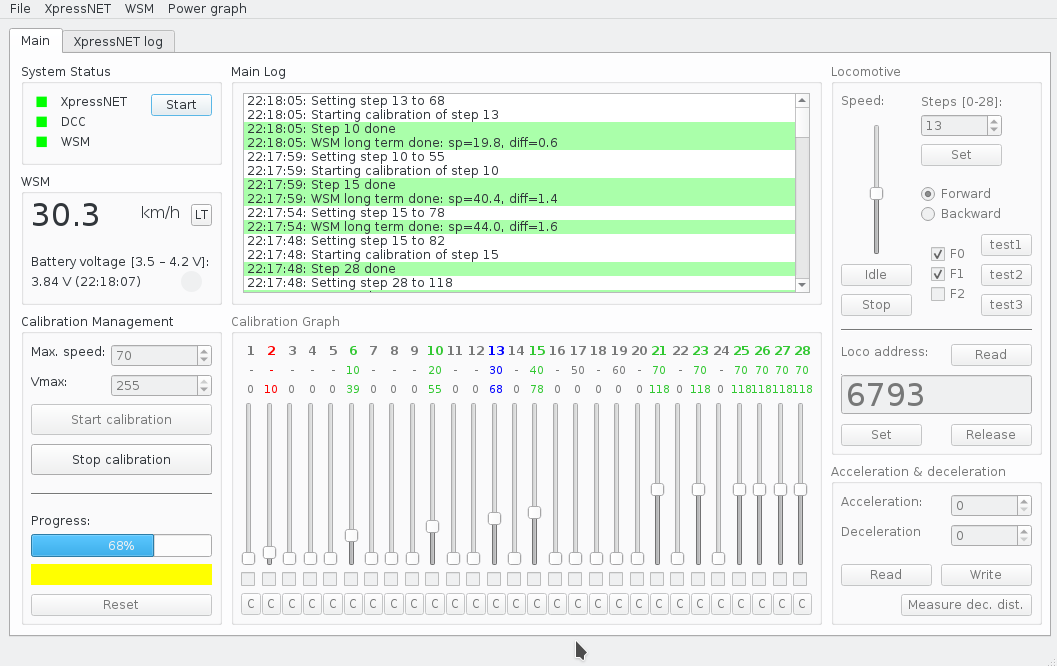
\includegraphics[width=\textwidth]{data/ac_progress.png}
\caption{Hlavní okno programu Automatic Calibration.}
\label{fig:ac-gui}
\end{figure}

Program je k~dispozici pod opensource licencí \textit{Apache License v2.0}
online\footnote{\url{https://github.com/kmzbrnoI/automatic-calibration}}.

Pro pochopení následujícího textu je třeba striktně rozlišovat několik pojmů:

\begin{enumerate}
\item \textit{Jízdní stupeň}

Jízdní stupeň je hodnota v~rozsahu $0$--$28$. Tuto hodnotu odesílá počítač
(nebo ovladač) do digitální centrály \gls{DCC} během ostrého provozu na kolejišti.
Centrála jízdní stupeň přeposílá do lokomotivy. Nastavením jízdního stupně
se řídí rychlost lokomotivy.

\item \textit{Otáčky přiřazené konkrétnímu jízdnímu stupni}

Otáčky motoru přiřazené konkrétnímu jízdnímu stupni se ukládají do \gls{CV} (viz
\ref{sec:trendy}) dekodéru a~mají mají rozsah $0$--$255$. Pro každý jízdní
stupeň je právě jedno \gls{CV}. Nastavení těchto \gls{CV} lze měnit jedině programováním
dekodéru a~neočekává se, že se při ostrém provozu bude do tohoto nastavení
zasahovat. Více jízdních stupňů může mít přiřazeno stejné otáčky.

\item \textit{Rychlost}

Rychlost je skutečná rychlost modelu měřená např. měřicím vozem. Rychlost
je svázaná s~otáčkami motoru, více jízdních stupňů může mít nastavené
stejné otáčky (a tudíž stejnou rychlost).

\end{enumerate}

Veškeré programování dekodéru v~lokomotivě probíhá v~režimu \textit{\gls{POM}}
(\textit{Programming on Main}), který umožňuje -- ačkoliv se nepředpokládá, že
se tato možnost využije -- programování za plného provozu
kolejiště.\footnote{\gls{DCC} centrála umí programovat dekodér ve dvou režimech:
(1)~programování na programovací koleji, (2)~\textit{Programming on Main -- \gls{POM}}.
Jedině na programovací koleji lze vyčítat \gls{CV}, při zvolení režimu \textit{\gls{POM}}
není možné přenášet data z~lokomotivy zpět do centrály, \gls{CV} lze tedy pouze
nastavovat. Lokomotiva ani nemůže potvrdit správné přijetí dat. Centrála ale
předem počítá s~případnou nespolehlivostí přenosu dat a~proto posílá
\textit{\gls{POM}} příkaz dekodéru několikrát. V~praxi se problém chybějící odezvy
neukazuje zásadní. Při programování na programovací koleji typicky není možný
provoz na kolejišti.} Režim \textit{\gls{POM}} byl zvolen zejména z~toho důvodu, že
při programování není lokomotivu nutné zastavovat (oproti programování na
programovací koleji), takže kalibrace rychlostí může být výrazně rychlejší.

Aplikace je vystavěna objektově. Je zde několik tříd založených na modelu
\textit{singleto}, kde každá třída má jednu konkrétní odpovědnost. Diagram
tříd je zobrazen na obrázku \ref{fig:ac-classes}, šipky reprezentují vztah
\textit{vlastní}.

\begin{figure}[ht]
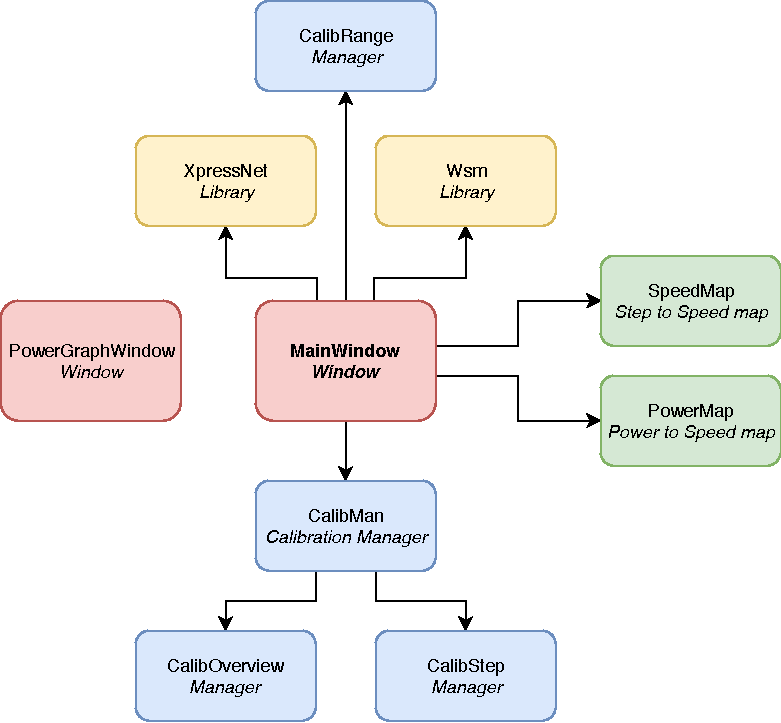
\includegraphics[width=0.7\textwidth]{data/ac_classes.pdf}
\caption{GUI programu \gls{WSM} Speed Reader.}
\label{fig:ac-classes}
\end{figure}

Kořenovou třídou je třída obsluhující hlavní okno (\texttt{MainWindow}),
v~projektu jsou dále knihovny umožňující komunikaci s~periferiemi (žluté třídy),
nad těmito knihovnami jsou správci kalibrace (modré třídy). V~projektu jsou
dále pomocné třídy (zelené obdélníky), které jsou využívány v~prakticky celé
aplikaci. Projekt je navržen tak, aby pouze červené třídy byly propojené
s~GUI, zbylé třídy mezi sebou komunikují pomocí volání funkcí a~Qt signálů.

Třída \texttt{SpeedMap} udržuje mapu \textit{jízdní stupeň: žádaná rychlost},
třída \texttt{Power\-Map} pak udržuje mapu \textit{otáčky motoru: naměřená rychlost}.

O~kalibraci rychlostních křivek se stará třída \texttt{CalibMan}. Kalibrace
je rozdělena do čtyřech fází.

\begin{compactenum}
\item Zapsání základních \gls{CV}.
\item Vytvoření základního přehledu o~závislosti \textit{otáčky motoru: rychlost}.
\item Kalibrace jednotlivých jízdních stupňů.
\item Interpolace zbylých jízdních stupňů.
\end{compactenum}

Kalibraci je kdykoliv možné přerušit, čímž dojde k~zastavení právě prováděné
operace a~k~zastavení hnacího vozidla. Protože si ale program pamatuje svůj
stav, je možné kalibraci kdykoliv spustit znovu a~již dokončené fáze jsou
přeskočeny.

Před začátkem kalibrace je nutné mít v~SW načtenou mapu \textit{jízdní
stupeň: žádaná rychlost} (viz přílohu \ref{fig:step-to-speed}). Tato mapa je
načítána z~\texttt{csv} souboru a~je možné definovat v~ní všechny, či pouze
vybrané jízdní stupně. Zbylé jízdní stupně se interpolují ze sousedních
nakalibrovaných hodnot nebo je nastaví uživatel manuálně. Tato mapa je
dohodnutou vlastností kolejiště a~typicky se nemění, proto se načítá z~jediného
souboru.

Před kalibrací navíc uživatel zadá \textit{maximální kalibrovanou rychlost}.
Tato rychlost je vlastností konkrétního hnacího vozidla, proto je možné ji
ovlivnit před každou jednotlivou kalibrací. Maximální rychlost spolu
s~akcelerací a~decelerací a~oběma mapami jsou ukládány do \texttt{xml} souboru
definice hnacího vozidla. Formát tohoto souboru byl záměrně převzat ze SW JMRI
\cite{jmri:web}, aby bylo možné soubory mezi programy přenášet.

Další parametry, jako je například umístění zařízení sériového portu centrály
či maximální povolená odchylka kalibrace, jsou načítány z~jediného
konfiguračního souboru formátu \texttt{ini}.

\subsection{Měření rychlosti}
\label{sec:ac:lt-measure}

Měření rychlosti v~průběhu kalibrace probíhá ve speciálním režimu \textit{\gls{LT} --
Long Term Measure}. Tento speciální režim je implementován v~knihov\-ně pro komunikaci
s~měřicím vozem a~umožňuje průměrování více naměřených rychlostí. Bystrý čtenář si
jistě všimne, že autor právě představuje druhou vrstvu průměrování dat
z~měřicího vozu (první probíhá již přímo ve vozu). Ano, je to tak. Ovšem cílem
průměrování na úrovní SW není pouze eliminovat oscilace rychlosti, výstupem
je totiž kromě průměrné rychlosti také rozdíl $v_{max} - v_{min}$ v~měřeném
intervalu. Tento \uv{pseudorozptyl} umožňuje kalibračnímu SW rozhodnout, kdy
je a~kdy není měření relevantní. A~přesně to kalibrační SW dělá.

Průměrování typicky probíhá pro $30$ naměřených rychlostí, tedy po dobu $3$~s.

Kdykoliv je rozdíl $v_{max} - v_{min}$ naměřených rychlostí příliš velký
(konstanta je konfigurovatelná, výchozí hodnota je $3$~km/h), je
měření ignorováno a~inicializováno měření nové. Pokud se nepovede změřit
rychlost několikrát (opět konfigurovatelná konstanta), proces kalibrace je
přerušen. Velký rozptyl rychlostí může být způsoben například nekvalitním
vozidlem (a takové vozidlo prostě odmítneme zkalibrovat) nebo například
členitostí trati -- přítomností oblouků, stoupání a~klesání, s~kterými se \gls{BEMF}
nevyrovná.

\subsection{Fáze kalibrace rychlosti}

\subsubsection{Zapsání základních \gls{CV}}

V~této krátké fázi program nastaví do lokomotivy základní \gls{CV}. Vypne rozjezdy
a~dojezdy a~nastaví škálovací parametry rychlostních křivek\footnote{Některé
dekodéry umožňují kromě přiřazení otáček každému stupni navíc zadat parametr,
který určuje, jaké reálné střídě signálu odpovídá maximální hodnota otáček.
Tím chtějí umožnit škálovat celou rychlostní tabulku bez nutnosti změnit otáčky
odpovídající každému jízdnímu stupni.} tak, aby hodnoty otáček $0$--$255$
reálně pokrývaly celé spektrum stříd signálů do motoru.

O~tento krok se stará přímo třída \texttt{CalibMan}.

\subsubsection{Vytvoření přehledu}

O~tento krok se stará třída \texttt{CalibOverview}.
Lokomotivě je nastaven jízdní stupeň $2$ a~na tento stupeň je zapsána hodnota otáček
$10$. Následně proběhne měření rychlosti. Dokud je rychlost lokomotivy
neměřitelná (příliš malá), otáčky jsou postupně zdvojnásobovány a~do mapy
\textit{otáčky: rychlost} jsou přidávány nové záznamy. Jakmile se lokomotiva
rozjede na rychlost $> V_{min}$, program má informaci o~tom, která hodnota
otáček motoru odpovídá minimální rychlosti lokomotivy a~přechází do další fáze.

V~další fázi zkouší program otáčky v~intervalu $64$--$255$, dokud nenaměří
rychlost vyšší než je uživatelem zadaná maximální rychlost.

Nyní má program představu o~tom, které hodnotě otáček motoru odpovídá minimální
rychlost a~kterému maximální rychlost. Všechna měření rychlosti lokomotivy
probíhají v~režimu \textit{\gls{LT}} (viz kapitolu \ref{sec:ac:lt-measure}).

Pokud uživatel načte profil již změřené lokomotivy ze souboru a~v~tom\-to profilu
jsou body, které jsou vyžadovány, tato fáze je přeskočena. Kalibrace vozidla,
které už jednou bylo kalibrováno, je tedy rychlejší.

\subsubsection{Kalibrace jízdních stupňů}

Třída \texttt{CalibStep} umožňuje zkalibrovat jeden jízdní stupeň. Třída
\texttt{CalibMan} pak postupně volá třídu \texttt{CalibStep} dokud nejsou
zkalibrovány všechny jízdní stupně, které si uživatel přál zkalibrovat.

Kalibrace jednoho stupně probíhá následovně.

\begin{compactenum}
\item V~mapě \textit{otáčky: rychlost} jsou vyhledány (interpolovány) otáčky odpovídající
      kýžené rychlosti.
\item Otáčky jsou zapsány do lokomotivy k~právě kalibrovanému stup\-ni.
\item Čeká se $2\ s$ na změnu rychlosti lokomotivy.
\item Začne měření rychlosti v~režimu \textit{\gls{LT}}.
\item Naměřená hodnota je přidána do mapy \textit{otáčky: rychlost}.
\item Pokud je rychlost v~$\epsilon$ toleranci (konstantní konfigurovatelná hodnota)
      cílové rychlosti, krok je zkalibrován, jinak se přechází znovu na krok
      (1)\footnote{Všimněte si, že v~následující iteraci je zapsána jiná (přesnější)
      hodnota otáček, neboť došlo ke zpřesnění mapy \textit{otáčky: rychlost}.}.
\end{compactenum}

$\epsilon$ je ve výchozím nastavení $1\ km/h$.

Jakmile je zkalibrována rychlost, která je přiřazena více jízdním stupňům,
jsou i~tyto jízdní stupně nastaveny na právě zkalibrovanou hodnotu otáček.

Průběh kalibrace je průběžně zobrazován uživateli. Uživatel vidí, které
jízdní stupně jsou již zkalibrovány a~které ještě ne.

\subsubsection{Interpolace}

Po dokončení kalibrace všech stupňů načtených z~\texttt{csv} souboru jsou zbylé
stupně interpolovány.

Po této fázi zůstává typicky nezkalibrována minimální
rychlost\footnote{Měřicí vůz neumí dobře měřit hodně malé rychlosti.}, pro kterou
v~\textit{Klubu modelářů železnic Brno I} platí úzus, že je to taková nejnižší
rychlost, při které se hnací vozidlo již začne plynule pohybovat. Po dokončení
kalibrace tedy uživatel ručně vybere jízdní stupeň $1$ a~nastaví mu
požadované otáčky za současného pozorování pohybu vozidla.

Program se pak postará o~to, aby byly stupně do nejbližšího již zkalibrovaného
stupně interpolovány.

\subsection{Kalibrace dojezdů}

Po zkalibrování rychlosti následuje kalibrace dojezdů. Zde se autor nakonec
rozhodl pro poloautomatickou kalibraci a~to zejména z~toho důvodu, že kalibrace
dojezdů je již velmi rychlá.

Program uživateli umožní zadat hodnotu decelerace (\gls{CV} \#4) a~pak pomocí kliku
na jediné tlačítko změřit dojezd z~rychlosti $40$~km/h. Program tedy vozidlo
rozjede, chvíli počká na ustálení rychlost, pak vozidlu nastaví jízdní stupeň
$0$ a~pomocí měřicího vozu měří dráhu do zastavení. Vzdálenost pak vypíše
uživateli, který na základě ní může upravit hodnotu decelerace.

Akcelerace je pak typicky nastavena stejně jako decelerace (ale volba je plně
na uživateli).

\section{XpressNET knihovna}
\label{sec:xn-lib}

Fundamentálním nástrojem pro fungování aplikace \textit{Automatic Calibration}
je knihovna, která umožňuje komunikaci s~centrálou XpressNET. Přestože je tento
protokol ve střední Evropě hojně rozšířen, pro jazyk C++ autor nenašel žádnou
rozumnou knihovnu, která by umožňovala s~XpressNET centrálou komunikovat.

Autor tedy implementoval vlastní opensource a~robustní XpressNET knihovnu
s~potvrzováním příkazů z~centrály a~vyčlenil ji do samostatného
repozitáře\footnote{\url{https://github.com/kmzbrnoI/xn-lib-cpp-qt}}. Autor
pevně věří, že si tato knihovna najde uplatnění napříč modelářskou komunitou.
